\section{Method}
The experimental setup consisted of an X-ray source pointing on a sample of powdered crystal. The sample was placed on a diffractometer connected to a computer to control the placement of the sample. Behind the sample was a large area detector used to capture the diffraction rings. The setup can bee seen in \ref{fig:setup}
\begin{figure}[H]
    \centering
    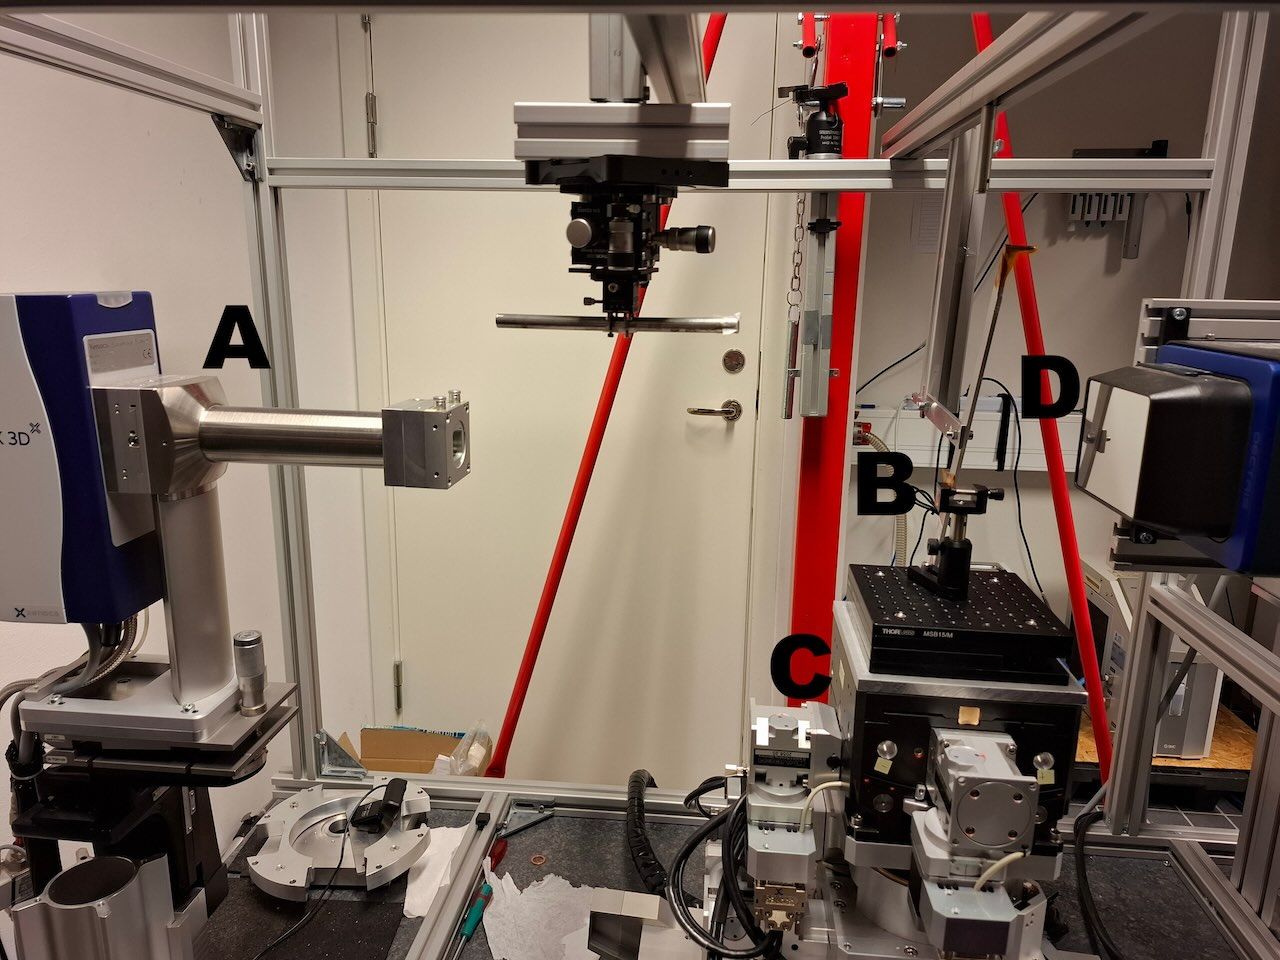
\includegraphics[width=0.7\textwidth]{Figures/setup_letters.jpg}
    \caption{The experimental setup. \textbf{A} is the X-ray source with X-ray energy of \SI{17.45}{\kilo\electronvolt}. \textbf{B} is the sample which were analysed. In the lab two different samples were tested. \textbf{C} is the diffractometer used to control the position of the sample. \textbf{D} is the detector made from six large semiconductors.}
    \label{fig:setup}
\end{figure}

During the lab the powders sample was put on the diffractometer, then the shutter on the X-ray source was opened, and the detector started recording. The diffractometer was controlled from the computer to move the sample until a diffraction pattern was seen in the detector. A 1-minute-long measurement were taken and the data saved. The process was repeated for the other sample as well.

Before analysing the data, the data was calibrated using the calibration sample LaB$_6$. The rings from the calibration sample were marked to calibrate the detector. During the analysis the data was masked to remove parts of the dead spots on the detector and hot spots where the detector was saturated. Then a 1D plot was generated from the 2D image to show the intensity as a function of the scattering angle. In some cases there were so called hot pixels, which are high peak intensities with no width. This is probably due to a pixel being burnt out, and these points were removed from the data.